\section{旋转建模法}
\subsection{绘制杯零件左视图}
\subsubsection{直接绘制法}\label{sec:beilingjianleft}
\begin{procedure}

\item 启动AutoCAD软件

爸爸:秦奋,我们首先要启动AutoCAD软件,你来说说有哪些启动方法。

秦奋:启动AutoCAD软件的方法通常有:
\begin{itemize}
\item 双击桌面图标
\includegraphics[scale=0.2]{cadicon.png}。
\item 【开始】菜单【所有程序】子菜单中【Autodesk】子菜单中【AutoCAD 2013 – 简体中文 (Simplified Chinese)】子菜单中的【AutoCAD 2013 – 简体中文 (Simplified Chinese)】项。
\end{itemize}
秦奋一边说一边进行操作,经过稍适等待,完成了AutoCAD软件的启动,出现了如图\ref{fig:cadui}所示的软件界面。
\noindent
\begin{figure}[htbp]
\centering
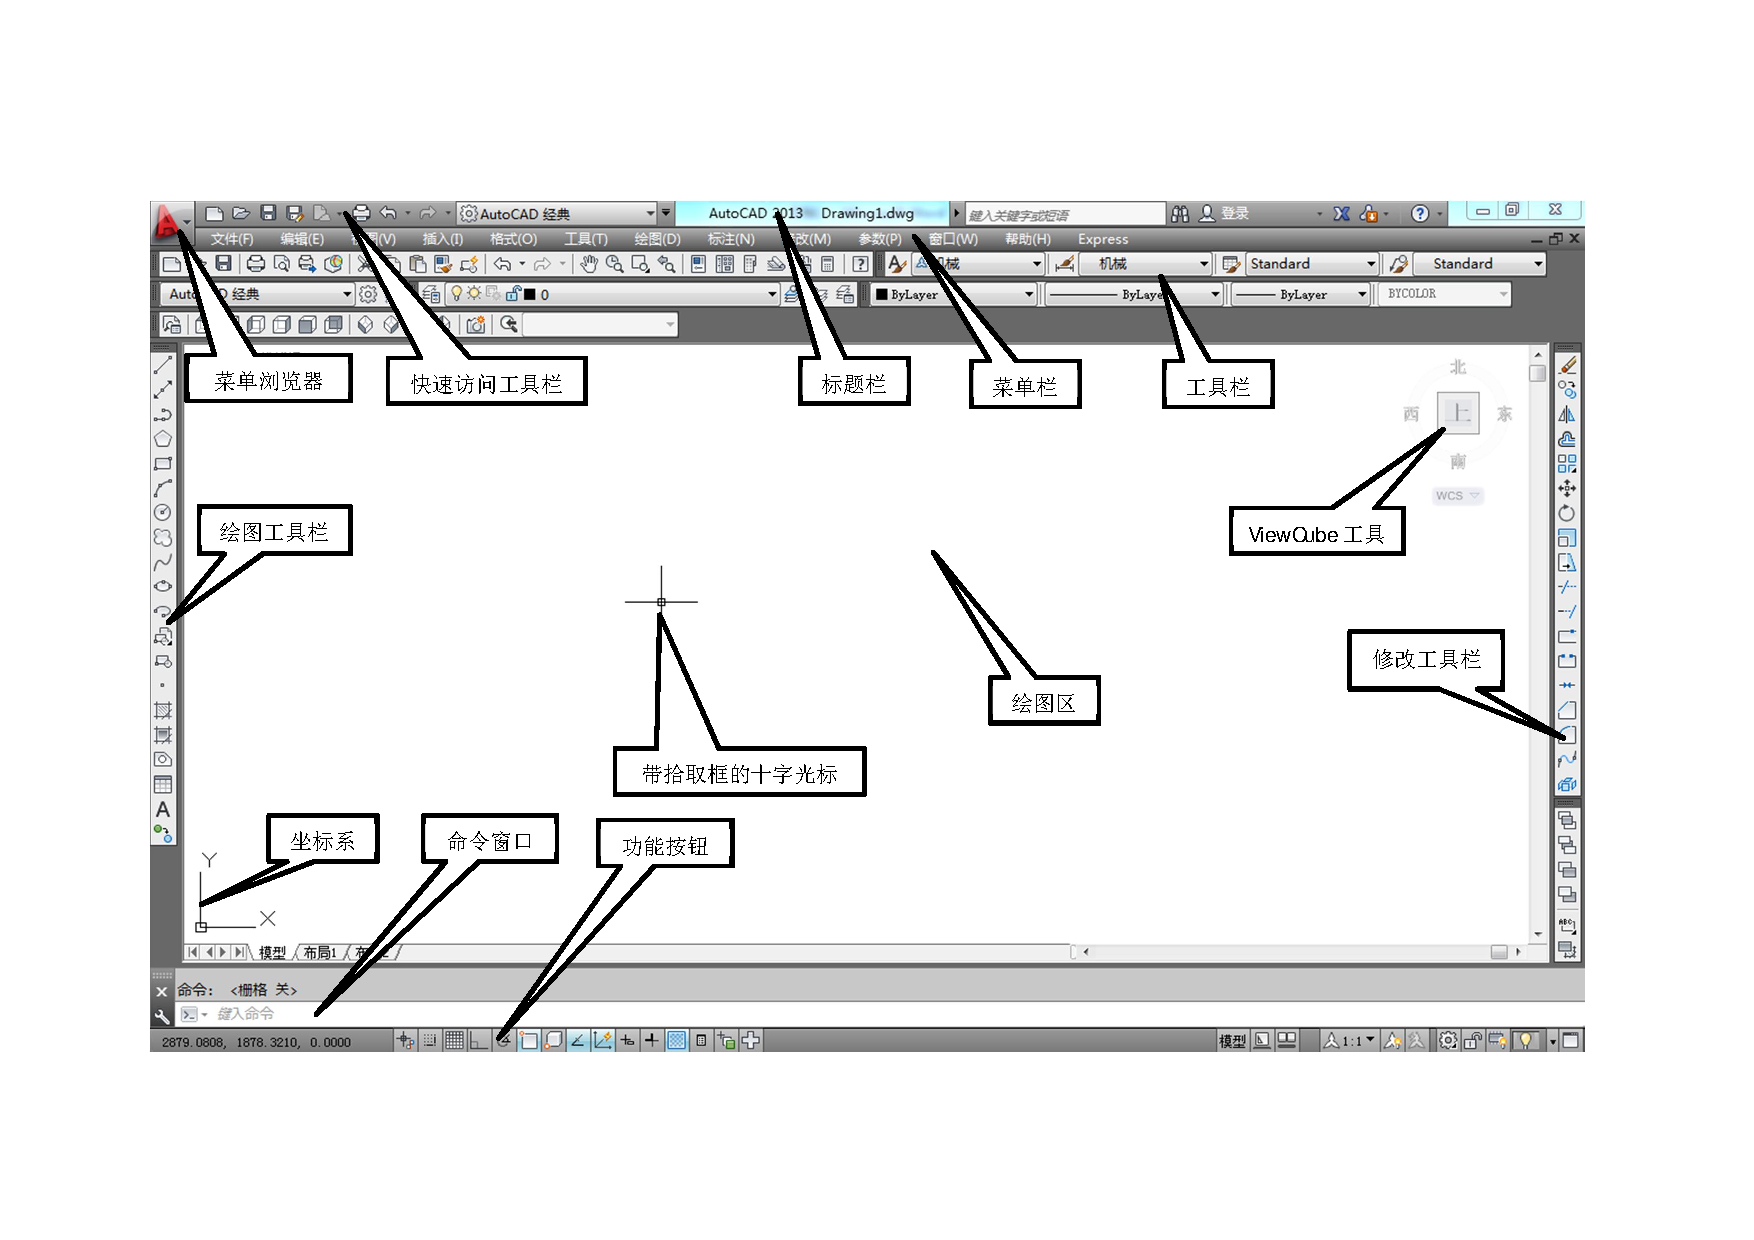
\includegraphics[scale=0.5]{cadui.pdf}
\caption{“AutoCAD经典”工作空间}\label{fig:cadui}
\end{figure}
爸爸指着软件的界面简单地介绍到:AutoCAD软件的界面同Word字处理软件的界面基本上差不多,有标题栏、菜单栏、工具栏、绘图区、状态栏。不同的是在标题栏上还有菜单浏览器和快速访问工具栏;绘图区的左下方还有坐标系,右上方有ViewCube工具,左边有绘图工具栏,右边有编辑工具栏;状态栏的上方有命令窗口;状态栏中还有按钮。

秦奋一边听一边默默地记着。
\item 将视图切换为左视图。

爸爸:AutoCAD启动后其默认的视图方向是主视图方向,为了方便使用旋转法进行杯零件的三维建模,我们需要将AutoCAD的视图方向切换为左视图方向。通常实现左视图切换的方法有:
\begin{itemize}
\item 键盘输入-VIME或-V,选择【正交】选项中的【左视】项。
\item 在【视图】菜单【三维视图】子菜单中单击【左视图】项。
\item 在【视图】工具栏中单击【左视】图标
\includegraphics[scale=0.6]{toptool.png}。
\end{itemize}
秦奋:是不是切换其它视图方向的方法也是基本一致的,只是需要将“左视”换成其它视图方向即可,如切换为俯视图方向是则将【左视】改为【俯视】,将【左视图】改为【俯视图】?

爸爸:不错,能够举一反三。

秦奋:为什么本例要使用左视图而不用主视图或其它视图呢?

爸爸:问得不错,因为我们接下来要绘制左视图中带有阴影部分的图形的边框线,因此需要切换到左视图,以便于得到我们期望的三维模型。其实我们在建模过程中经常需要切换视图方向以利于建模。

秦奋:那就是说,如果绘制的图框位于主视图,寻么就需要将视图方向切换为主视图。

爸爸:嗯,不错,看来你已经理解了视图切换的意义的目的了。接下来我们就要开始绘图了。
\item 启动【直线】命令

爸爸:秦奋你观察一下左视图的边框线都有是些什么线?

秦奋:都是由直线围成的。

爸爸:因此我们可以用AutoCAD中的【直线】命令来完成阴影部分的边框线绘制。【直线】命令的常用启动方法有以下几种:
\begin{itemize}
\item 键盘输入line或L。
\item 在【绘图】菜单中单击【直线】项。
\item 在【绘图】工具栏中单击【直线】图标
\includegraphics[scale=0.6]{linetool.png}。
\end{itemize}
此时秦奋的爸爸在命令窗口中输入了【直线】命令。
\begin{lstlisting}
|命令: LINE|
|指定第一个点:
\end{lstlisting}
爸爸:秦奋,注意到绘图区和命令窗口的变化了吗?

秦奋:输完命令后绘图区中的光标由带拾取框的十字光标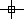
\includegraphics[scale=0.8]{guangbiao1} 变成了十字光标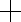
\includegraphics[scale=0.6]{guangbiao2}。命令窗口中提示输入第一个点。

爸爸:这种状态是AutoCAD系统提示我们需要输入直线第一个点坐标。通常有三种方式输入坐标:
\begin{itemize}
\item 坐标数字
\item 光标直接输入
\item 光标捕捉方式输入
\end{itemize}

其中坐标数字和光标捕捉方式能够获得精确的坐标位置,而光标直接输入的坐很不准确。精确绘图是AutoCAD的主要特色,因此用光标直接输入的方式应用比较少。
\item 输入图线坐标点,实现封闭图形的绘制。

秦奋的爸爸快速的完成了左视图边框的绘制。
\begin{lstlisting}
|指定第一个点:0,0|
|指定下一点或 [放弃(U)]: 15<0|
|指定下一点或 [放弃(U)]: $@4<90$|
|指定下一点或 [闭合(C)/放弃(U)]: $@-10<0$|
|指定下一点或 [闭合(C)/放弃(U)]: $@11<90$|
|指定下一点或 [闭合(C)/放弃(U)]: $@-5<0$|
|指定下一点或 [闭合(C)/放弃(U)]: c|
\end{lstlisting}

爸爸:通过上述步骤,我们完成了杯零件的主要特征绘制,其结果如图\ref{fig:bettezheng}所示。现对步骤中标注部分说明如下:
%\showremarks
\noindent
\begin{figure}[htbp]
\centering
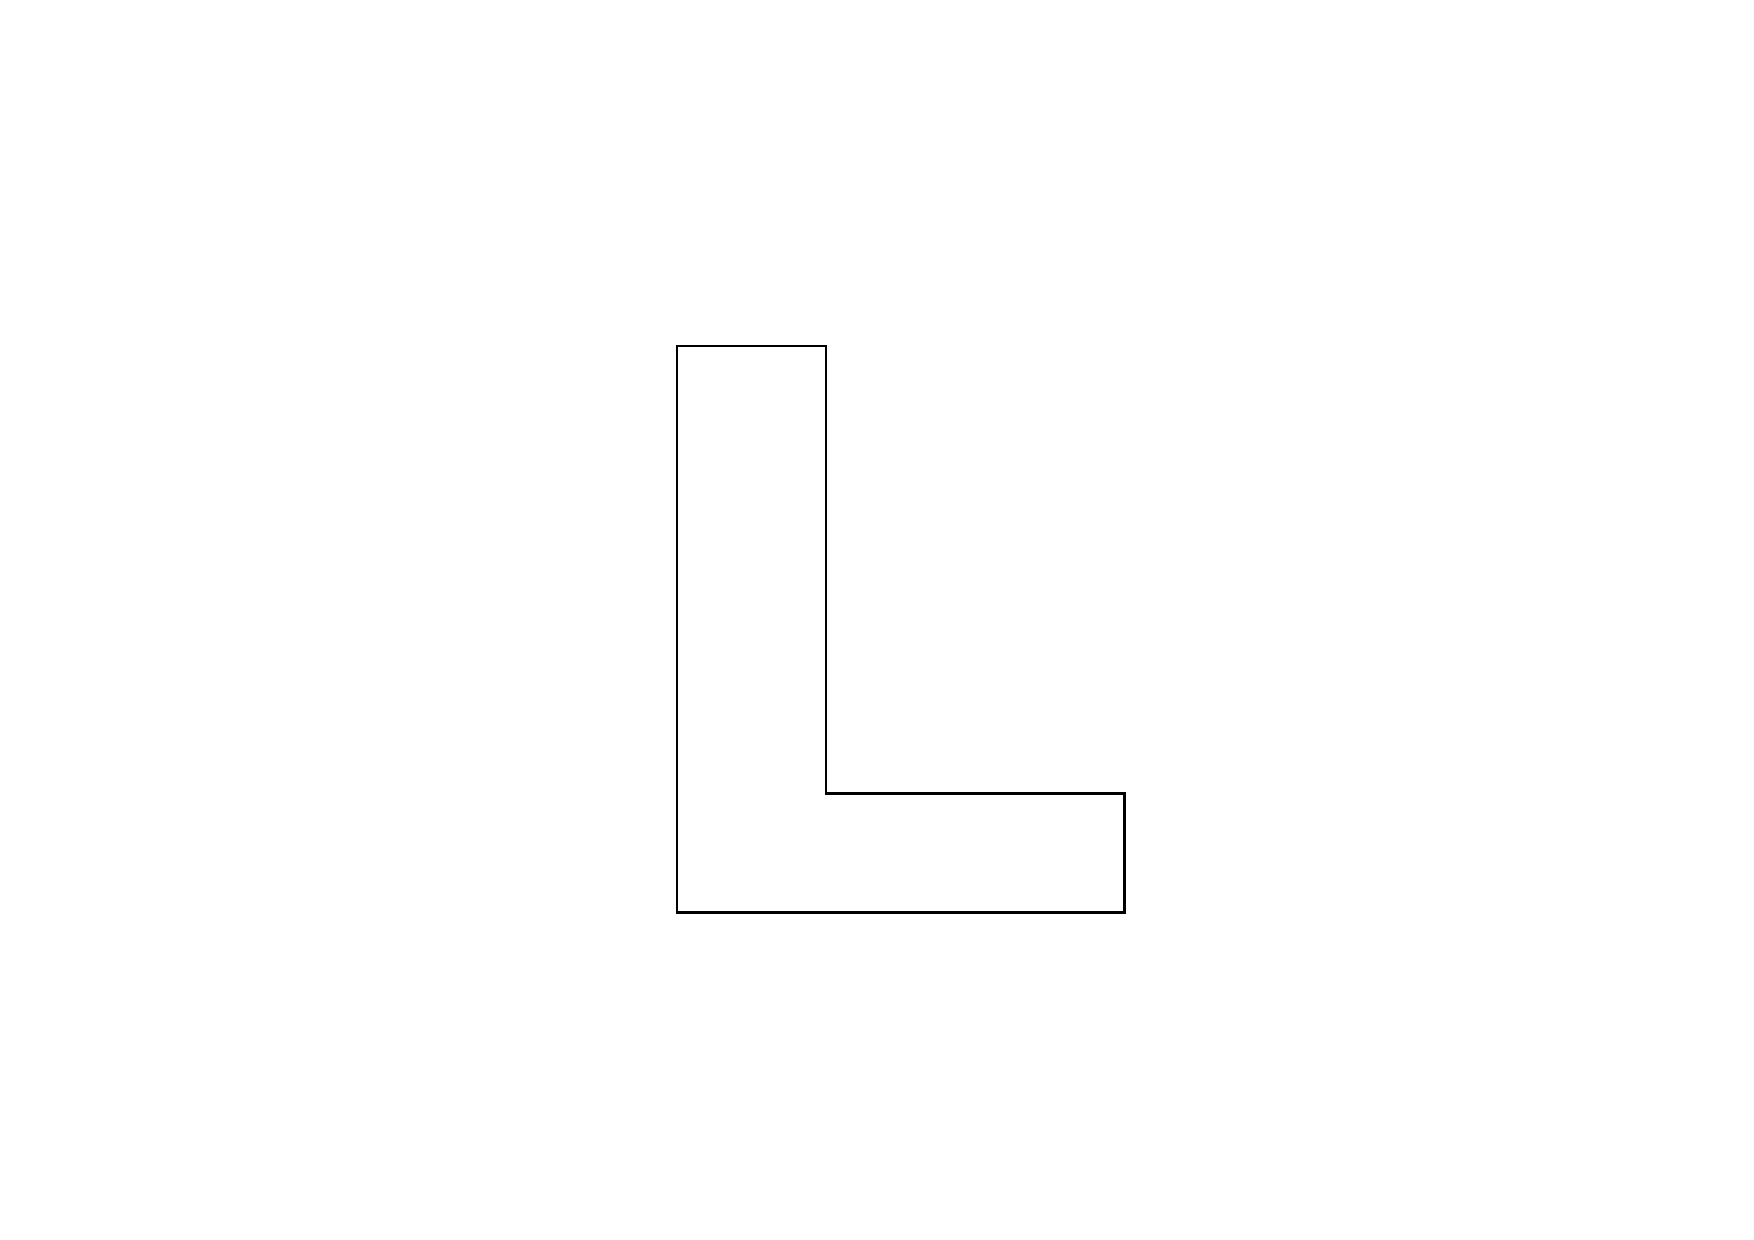
\includegraphics[scale=0.4]{beitezheng.pdf}
\caption{杯零件三维建模基础图}\label{fig:bettezheng}
\end{figure}
\end{procedure}

\subsubsection{坐标知识}
秦奋:为什么四种不同的坐标数字表达形式呢,它们之间有什么区别呢。

爸爸:坐标是精确定位AutoCAD对象的基础,在上面(第\ref{sec:beilingjianleft}节)的绘图过程中我们使用四种不同的坐标表示方法,它们分别是绝对直角坐标、相对直角坐标、绝对极轴坐标和相对极轴坐标。其中绝对直角坐表示法就是我们在数学中所学的直角坐标表示法,在AutoCAD软件中称为世界坐,其表示形式为$(x,y)$,图\ref{fig:zuobiao1}中的$(0,0)$和$(2,1)$即为绝对坐标表示。。相对直角坐标表示则是将图形中的某一点假设为坐标原点,并以此为参照表示图形中的其它点的表示方法,在AutoCAD中用$(@x,y)$的形式进行表示,图\ref{fig:zuobiao1}中的$(@2,1)$即为将$(2,1)$假设为坐标原点$(0',0')$进行表示的,可以容易地看出其值分别是相对于假设原点的$x$和$y$坐标增量。绝对极轴坐标表示法是用点与点之间的线段长度以及该连线与水平线之间的夹角来表示点的具体位置,在AutoCAD中用$(@$距离$<$角度$)$的形式表示,图\ref{fig:jizuobiao1}中的$(0<0\degree)$为极轴坐标的原点表示,$(1<45\degree)$为点在绝对极轴坐标中的位置表示。相对极轴坐标表示法与相对直角坐标表示类似,也是以将图形中的某一点假设为极轴坐标原点,并将其作为参考来表示图形中的其它点的位置。绝对直角坐标和绝对极轴坐标表示都要求准确地给出物体每一个点的准确位置,对于简单的图形是可行的,但对于复杂的图形,其计算量比较大,不能够满足快速绘图的需要。相对直角坐标和相对极轴坐标表示通常是用增量进行表示,因此计算简单、直观,较好地满足了快速绘图的需要。四种坐标表示方式需要根据绘制图形的需要进行选择,以方便表达减少计算量为目标。
\begin{figure}[htbp]
\centering
\begin{floatrow}
\ffigbox{\caption{直角坐标表示}\label{fig:zuobiao1}}{
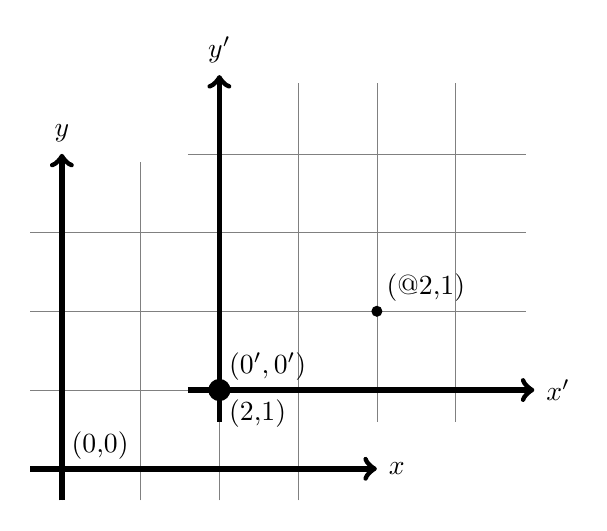
\begin{tikzpicture}
\draw[help lines,step=1cm,very thin](-0.4cm,-0.4cm)grid(3.9cm,3.9cm);
\draw[->,line width=0.7mm](-0.4cm,0)--(4cm,0)node[right]{$x$};
\draw[->,line width=0.7mm](0,-0.4cm)--(0,4cm)node[above]{$y$};
\draw (0,0)node[above right]{(0,0)};
\fill (2cm,1cm)node[below right]{(2,1)}circle(4pt);
\begin{scope}[shift={(2cm,1cm)}]
\draw[help lines,step=1cm,very thin](-0.4cm,-0.4cm)grid(3.9cm,3.9cm);
\draw[->,line width=0.7mm](-0.4cm,0)--(4cm,0)node[right]{$x'$};
\draw[->,line width=0.7mm](0,-0.4cm)--(0,4cm)node[above]{$y'$};
\draw (0,0)node[above right]{$(0',0')$};
\fill (2cm,1cm)node[above right]{(@2,1)}circle(2pt);
\end{scope}
\end{tikzpicture}}
\ffigbox{\caption{极轴坐标表示}\label{fig:jizuobiao1}}{
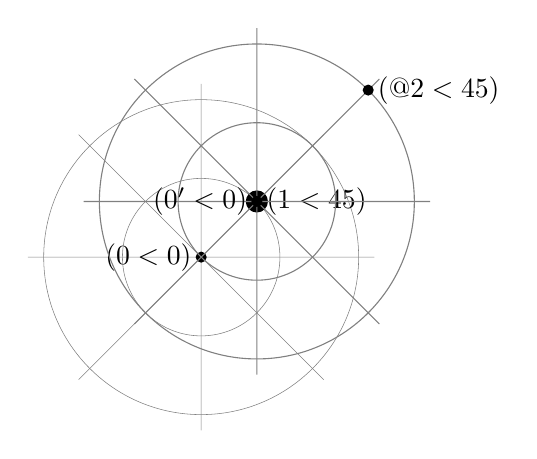
\begin{tikzpicture}
\draw[help lines,very thin](-2.2cm,0)--(2.2cm,0)(0,-2.2cm)--(0,2.2cm)(45:2.2cm)--(225:2.2cm)(135:2.2cm)--(-45:2.2cm);
\fill(0,0)node[left]{($0<0\degree$)}circle(2pt);
\draw[help lines,very thin](0,0)circle(1cm)circle(2cm);
\fill (45:1cm)node[above,right]{$(1<45\degree)$}circle(4pt);
\begin{scope}[shift={(45:1cm)}]
\draw[help lines,thin](-2.2cm,0)--(2.2cm,0)(0,-2.2cm)--(0,2.2cm)(45:2.2cm)--(225:2.2cm)(135:2.2cm)--(-45:2.2cm);
\draw[help lines,thin](0,0)circle(1cm)circle(2cm);
\fill (45:2cm)node[right]{$(@2<45\degree)$}circle(2pt);
\fill(0,0)node[below,left]{($0'<0\degree$)}circle(2pt);
\end{scope}
\end{tikzpicture}
}
\end{floatrow}
\end{figure}
\subsubsection{直线命令使用技巧}
秦奋:如果在绘制的过程中如果出现了错误或意外中结束了命令该怎么办呢?

爸爸:其实在绘图过程中,我们不可能不出现操作失误。现在我就告诉你一些直线命令使用过程中的技巧。
\begin{tips}
\item 在使用Line命令的过程中,如果由于输入坐标错误或误点鼠标而导线段绘制错误,只要没有结束命令,可以直接输入U来撤消上一次绘制的线段。
\item 在使用Line命令过程中,如果还没有完成图形的绘制就提前结束了命令,可以再次使用直线命令,并利用端点捕捉的方式获得命令结束时所绘制端点的坐标,然后接着完成图形的绘制。开启端点捕捉的方法有:
\begin{itemize}
\item 绘图过程中在输入坐标点的地方用键盘输入:end。
\item 绘图过程中按ctrl或shift键+鼠标右击弹出图\ref{fig:duixiangbuzuomen2}所示的【对象捕捉】菜单,并选择【端点】项。
\item 在功能按钮区中将对象捕捉图标由
\includegraphics[scale=0.6]{duixiangbuzuo1.png}状态设置为
\includegraphics[scale=0.6]{duixiangbuzuo.png}状态,并在图标上右击弹出图\ref{fig:duixiangbuzuomen1}所示的【对象捕捉】菜单,并使【端点】项为开启状态。
\end{itemize}
\item 直线命令的C选项用于将最后一点与第一点连接起来并结束命令。
\item 使用坐标和捕捉是实现AutoCAD精确绘图的关键。
\end{tips}
\begin{figure}[htbp]
\centering
\begin{floatrow}
\ffigbox{\caption{“对象捕捉”菜单一}\label{fig:duixiangbuzuomen2}}{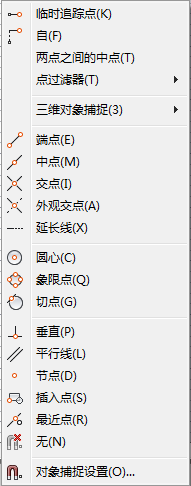
\includegraphics[scale=0.85]{duixiangbuzuomen2.png}}
\ffigbox{\caption{“对象捕捉”菜单二}\label{fig:duixiangbuzuomen1}}{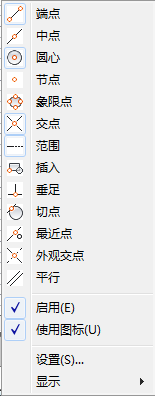
\includegraphics{duixiangbuzuomen1.png}}
\end{floatrow}
\end{figure}
爸爸:你先来练习一下。

秦奋很快地绘制完了图形。他父亲对他的整个绘图过程很满意。

\subsubsection{修剪法}
秦奋:绘制杯零件图的特征图还有别的方法吗?

爸爸:在AutoCAD中完成同样的图形绘制通常有多种不同的方法,其实绘制图\ref{fig:bettezheng}所示的图形,还可以用修剪的方法获得。这种方法的核心是先绘一些简的线或图形,然后通过编辑修改得到想要的图形。用修剪法绘制图\ref{fig:bettezheng}的步骤为:
\begin{procedure}
\item 绘制两条相互垂直的直线,作为基础。
\begin{lstlisting}
|命令: LINE|
|指定第一个点:0,15|
|指定下一点或 [放弃(U)]: @0,-15|
|指定下一点或 [放弃(U)]: $@15<0$|
|指定下一点或 [闭合(C)/放弃(U)]: |
\end{lstlisting}
\item 用偏移产生符合尺寸距离的水平线。启动【偏移】命令的方法有:
\begin{itemize}
\item 键盘输入OFFSET或O。
\item 在【修改】菜单中单击【偏移】项。
\item 在【修改】工具栏中单击【偏移】图标
\includegraphics[scale=0.6]{offsettool.png}。
\end{itemize}
启动【偏移】命令后,AutoCAD要求指定图形的偏移距离。
\begin{lstlisting}
|命令:OFFSET|
|当前设置: 删除源=否  图层=源  OFFSETGAPTYPE=0|
|指定偏移距离或 [通过(T)/删除(E)/图层(L)] $<$通过$>$:  4|
\end{lstlisting}
指定偏移距离后,要求选择用于偏移的对象,此时用鼠标选择图\ref{fig:trimmotherd}中的水平线,选中后该水平线将以虚线形式表示,如图\ref{fig:offsetselect}所示。
\begin{lstlisting}
|选择要偏移的对象,或 [退出(E)/放弃(U)] $<$退出$>$:|
\end{lstlisting}
接下来,要求指定图形向哪一侧偏移,此时将鼠标移至选中水平线的上方,并单击鼠标左键,即完成一次图形的偏移操作。
\begin{lstlisting}
|指定要偏移的那一侧上的点,或[退出(E)/多个(M)/放弃(U)]|
|$<$退出$>$:|
|选择要偏移的对象,或 [退出(E)/放弃(U)] $<$退出$>$:|
\end{lstlisting}
然后,再用相同的方法得到另一条水平线。
\begin{lstlisting}
|命令: OFFSET|
|当前设置: 删除源=否  图层=源  OFFSETGAPTYPE=0|
|指定偏移距离或 [通过(T)/删除(E)/图层(L)] $<4.0000>$:  11|
|选择要偏移的对象,或 [退出(E)/放弃(U)] $<$退出$>$:|
|指定要偏移的那一侧上的点,或 [退出(E)/多个(M)/放弃(U)] |
|$<$退出$>$:|
|选择要偏移的对象,或 [退出(E)/放弃(U)] $<$退出$>$:|
\end{lstlisting}

\item 用偏移产生符合尺寸距离的垂直线。
\begin{lstlisting}
|命令:OFFSET|
|当前设置: 删除源=否  图层=源  OFFSETGAPTYPE=0|
|指定偏移距离或 [通过(T)/删除(E)/图层(L)] $<11.0000>$:  5|
|选择要偏移的对象,或 [退出(E)/放弃(U)] $<$退出$>$:|
|指定要偏移的那一侧上的点,或[退出(E)/多个(M)/放弃(U)]|
|$<$退出$>$:|
|选择要偏移的对象,或 [退出(E)/放弃(U)] $<$退出$>$:|
|命令: OFFSET|
|当前设置: 删除源=否  图层=源  OFFSETGAPTYPE=0|
|指定偏移距离或 [通过(T)/删除(E)/图层(L)] $<5.0000>$:  10|
|选择要偏移的对象,或 [退出(E)/放弃(U)] $<$退出$>$:|
|指定要偏移的那一侧上的点,或 [退出(E)/多个(M)/放弃(U)] |
|$<$退出$>$:|
|选择要偏移的对象,或 [退出(E)/放弃(U)] $<$退出$>$:|
\end{lstlisting}
\begin{figure}[htbp]
\subfloat[]{\label{fig:trimmotherd}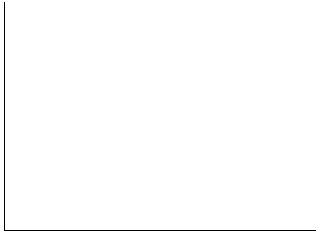
\includegraphics[scale=0.4]{trimmotherd1.png}}\hspace{20pt}
\subfloat[]{\label{fig:offsetselect}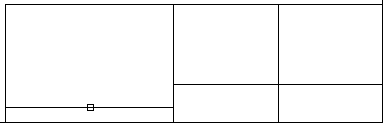
\includegraphics[scale=0.4]{offsetselect.png}}\hspace{20pt}
\subfloat[]{\label{fig:offsetresult}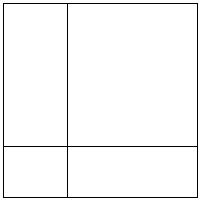
\includegraphics[scale=0.5]{offsetresult.png}}
\caption{偏移过程}
\end{figure}
\item 修剪图形。

在完成偏移操作后,其结果如图\ref{fig:offsetresult}所示,需要用【修剪】命令修剪掉多余的线段,以获得需要的图形。【修剪】命令的启动方法有:
\begin{itemize}
\item 解盘输入TRIM或TR。
\item 点击【修改】菜单中的【修剪】项。
\item 点击【修改】工具栏中的【修剪】图标
\includegraphics[scale=0.6]{trimtool.png}。
\end{itemize}
启动修剪命令后要求指定用于修剪的边,其命令提示为:
\begin{lstlisting}
|命令: TRIM|
|当前设置:投影=UCS,边=无|
|选择剪切边...|
\end{lstlisting}
此时,我们可以用框选方式选择所有的图线用作剪切边,选择方法如图\ref{fig:trimegeselect}所示,选择结果如图\ref{fig:trimselectresult}所示。其命令提示为:
\begin{lstlisting}
|选择对象或 $<$全部选择$>$:  指定对角点: 找到 6 个|
|选择对象:|
\end{lstlisting}
结束修剪边的选择后,要求我们选择要修剪的线段或者图形。我们同样用框选方式选择要修剪的对象,选择方法如图\ref{fig:trimedselect}所示,修剪完成后,其结果如图\ref{fig:trimedresult}所示。其命令提示为:
\begin{lstlisting}
|选择要修剪的对象,或按住 Shift 键选择要延伸的对象,或|
|[栏选(F)/窗交(C)/投影(P)/边(E)/删除(R)/放弃(U)]:  指定对角点:|
\end{lstlisting}
再用拾取的方式将剩下的多余的线段修剪掉,得到图\ref{fig:bettezheng}所示的图形。其命令提示为:
\begin{lstlisting}
|选择要修剪的对象,或按住 Shift 键选择要延伸的对象,或|
|[栏选(F)/窗交(C)/投影(P)/边(E)/删除(R)/放弃(U)]:|
|选择要修剪的对象,或按住 Shift 键选择要延伸的对象,或|
|[栏选(F)/窗交(C)/投影(P)/边(E)/删除(R)/放弃(U)]:|
|选择要修剪的对象,或按住 Shift 键选择要延伸的对象,或|
|[栏选(F)/窗交(C)/投影(P)/边(E)/删除(R)/放弃(U)]:|
\end{lstlisting}
\begin{figure}[htbp]
\subfloat[]{\label{fig:trimegeselect}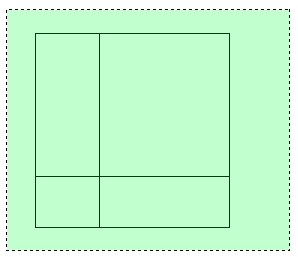
\includegraphics[scale=0.4]{trimegeselect.png}}\hspace{20pt}
\subfloat[]{\label{fig:trimselectresult}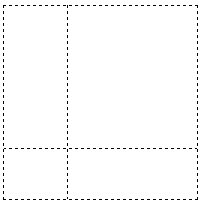
\includegraphics[scale=0.4]{trimselectresult.png}}\hspace{20pt}
\subfloat[]{\label{fig:trimedselect}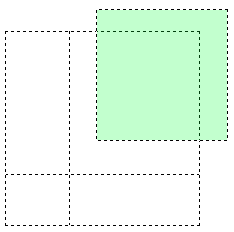
\includegraphics[scale=0.4]{trimedselect.png}}\hspace{20pt}
\subfloat[]{\label{fig:trimedresult}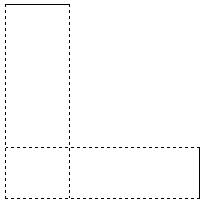
\includegraphics[scale=0.4]{trimedresult.png}}
\caption{修剪过程}
\end{figure}
\end{procedure}

秦奋:偏移命令和修剪命令使用过程中有哪些技巧呢?

爸爸:偏移命令和修剪命令的使用技巧有:
\begin{tips}
\item 【偏移】操作过程中,如果多次偏移的距离相同则可以多次选择对象并执行偏移。
\item 【修剪】操作的关键是修剪边的选择,若要剪去某线段之外的其它图线,则应选择该线段作为修剪边;若要剪去某两条线段之间的其它的图线则至少要选择该两条线段,否则不能够实现操作目的。
\item 【修剪】操作中修剪对象的选择具有一定的顺序,一般为先剪去外围不需要的图线,再剪去内部的图线,否会出现部分图线不能够剪除,只能够删除的现象。
\end{tips}

爸爸:你现在练习一下修剪法绘制图形。

秦奋用修剪法
\endinput